\documentclass[10pt,conference,compsocconf]{IEEEtran}
\usepackage{hyperref}
\usepackage{graphicx}
\usepackage{xcolor}
\usepackage{blindtext, amsmath, comment, subfig, epsfig }
\usepackage{caption}
\usepackage{algorithmic}
\usepackage{cite}
\usepackage[utf8]{inputenc}
\usepackage{csquotes}

\title{CS-523 Project 1 Report}
\author{Elvric Trombert, Francesco Intoci}
\date{February 2020}

\begin{document}

\maketitle

\begin{abstract}
    A scalable, flexible Secure Multi Party Computation framework with a trusted third party , designed for a semi-honest passive adversary.
\end{abstract}

\section{Introduction}
As described by \cite[Frikken]{Frikken2011}, Secure Multiparty Computation \enquote{allow for the distributed computation of a
function over distributed inputs without revealing additional information about the inputs, rather than what can be inferred from the output of the computation.}

In this project we have implemented an SMC framework relying on a trusted third party to coordinate communication between
parties, fulfilling tasks like delivering shares of one party secret to the other participants or storing the partial shares
of the circuit evaluation to be retrieved by the parties.

\section{Threat model}
In SMC the main goal of the adversary is to gain knowledge of the inputs used by the participants in the computation of
the function.
SMC model is secure against \textit{passive} adversaries, meaning that adversaries are capable of eavesdropping
the communication between parties and the server and of "corrupting" parties, gaining knowledge of their inputs, without deviating from the protocol.
Using additive secret
sharing, sampling the shares uniformly at random in $Z_q$ with $q$ prime, the model is information-theoretically secure against a passive \textit{MITM}.
Assuming $n-1$ dishonest parties collaborating to
infer the input of a target party, the framework results secure (most of the time) in this scenario.
A privacy problem arises when observing the circuit output: if the adversary is capable of gaining knowledge of $s-1$ out of $s$ secret inputs of the circuit, then retrieving the
target party's secret is easy as it involves solving a \textit{1-indeterminate} equation.
Note that the framework maintains the confidentiality of the target party's input even against an
\textit{active} adversary who can deviate from the protocol, but it can't ensure correctness.

\section{Implementation details}
The entry point of the protocol is represented by the \texttt{run} function of the \texttt{SMCParty class}.
This function will first invoke the \texttt{init\_secret\_sharing} function, which will handle the secret shares generation.
Once the shares are sent to the other parties via the server, the party calls the \texttt{process\_expression} function.
Expressions are represented by an AST, where each parent node is an operation and each leaf is an \texttt{operand}, i.e either a \texttt{Secret} or a \texttt{Scalar}.
To this purpose, we defined a new class, extending the \texttt{Expression} class, called \texttt{Operation}, which has two attributes, \texttt{a} and \texttt{b},
which are generic expressions (either another operation or an operand), and \texttt{operand\_type}, which is an Enum describing the kind of operation to be computed on the local values (i.e shares)
of the operands. \texttt{process\_expression} will then be invoked recursively on \texttt{a} and \texttt{b}.
The implementation of the protocols for addition and multiplication (\texttt{Add-K}, \texttt{Beaver Triplets}) follows the description in the course material.

\section{Performance evaluation}
All measurements were performed directly on each party and recorded.
The bytes in and out where measured on every
network call made by the party.
The runtime was measured as the time elapsed between the start of \texttt{run} function in
party\_smc.py and the time when that function returns.
Every individual case in each condition was run a total of 10 times.
Unless otherwise specified the number of parties involved in each test was 5.
Hence the total number of measurements for test case is : $n \times 10$, where $n$ is the number of parties.
Each plot describes the mean and the standard error of the measurement, represented by \texttt{matplotlib} 'errobars', and the variance (in some test case the error is too small to be plotted).
Tests were run on the following hardware: Intel core i7-7500U and Intel core i7-8565U. There was not any noticeable difference.

\begin{figure}[h!]
    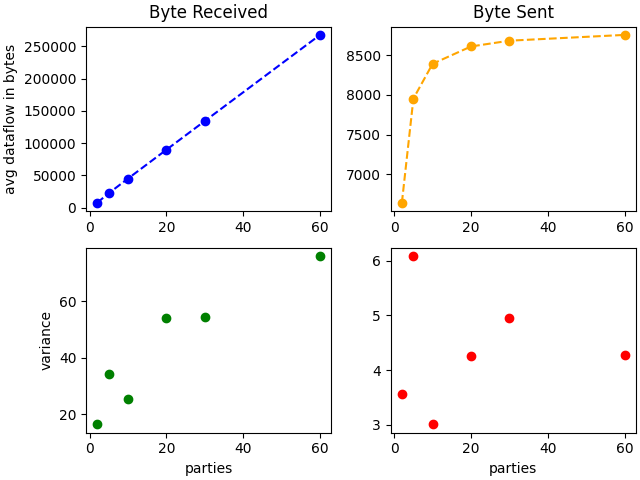
\includegraphics[width=0.49\linewidth]{../performance_analysis/dataflow_num_party_change.png}
    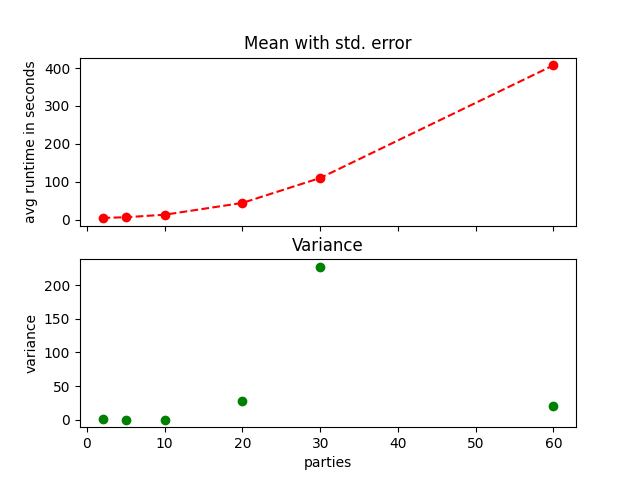
\includegraphics[width=0.49\linewidth]{../performance_analysis/runtime_num_party_change.png}
    \caption{Avg Runtime and Dataflow change based on the number of parties}
    \label{fig:num_parties}
\end{figure}


\begin{figure}[h!]
    \centering
    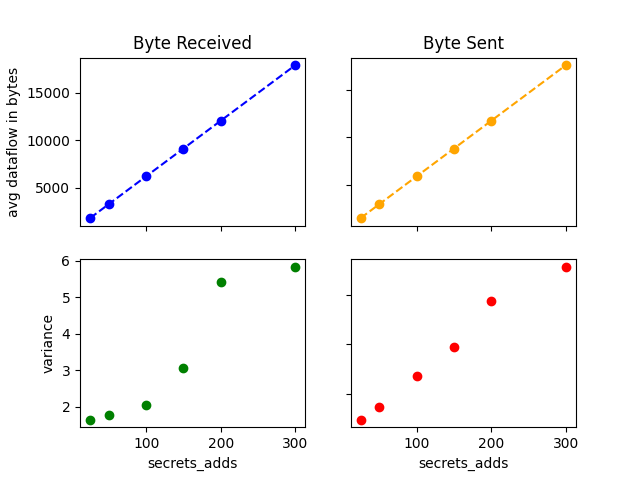
\includegraphics[width=0.49\linewidth]{../performance_analysis/dataflow_secrets_additions.png}
    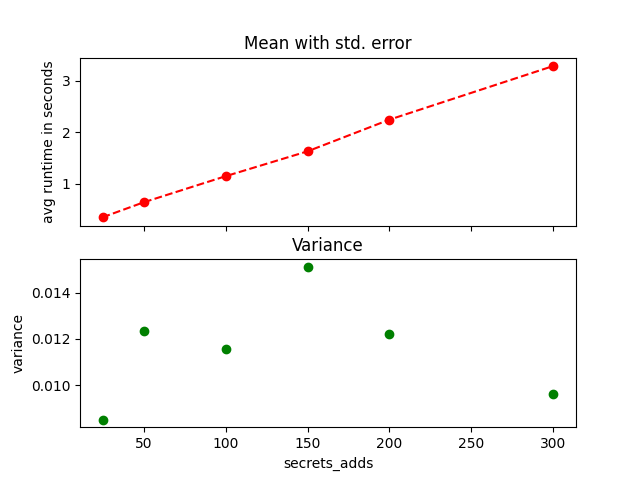
\includegraphics[width=0.49\linewidth]{../performance_analysis/runtime_secrets_additions.png}
    \caption{Avg Runtime and Dataflow change based on the number of Secret Addtions}
    \label{fig:num_additions}
\end{figure}

\begin{figure}[h!]
    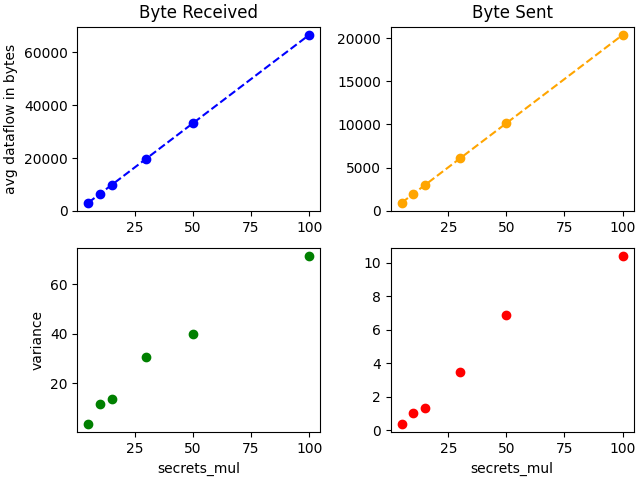
\includegraphics[width=0.49\linewidth]{../performance_analysis/dataflow_secrets_multiplications.png}
    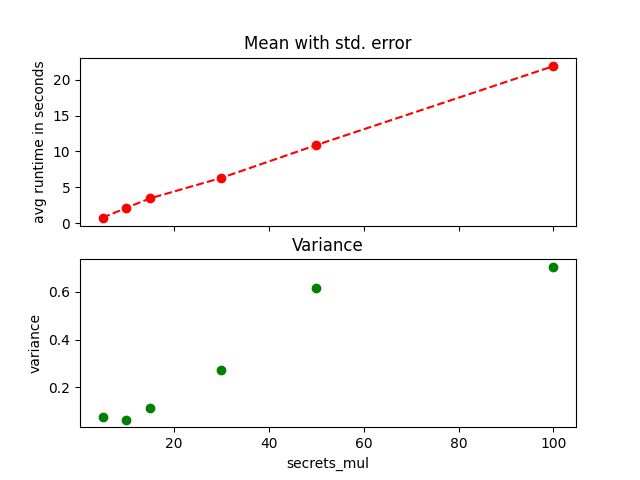
\includegraphics[width=0.49\linewidth]{../performance_analysis/runtime_secrets_multiplications.png}
    \caption{Avg Runtime and Dataflow change based on the number of Secret Multiplications}
    \label{fig:num_multiplications}
\end{figure}

\begin{figure}[h!]
    \centering
    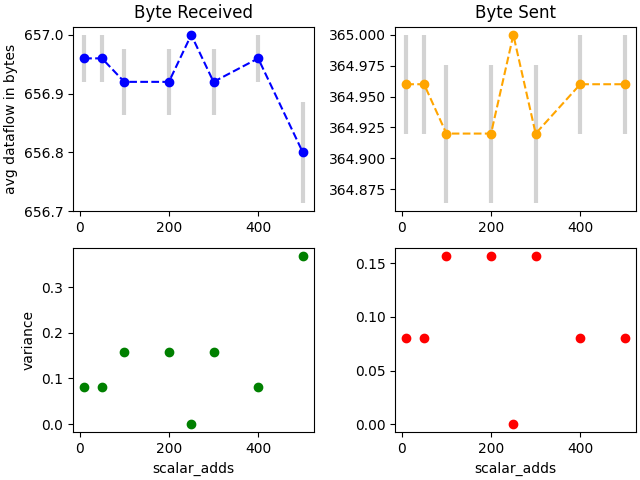
\includegraphics[width=0.49\linewidth]{../performance_analysis/dataflow_scalar_additions.png}
    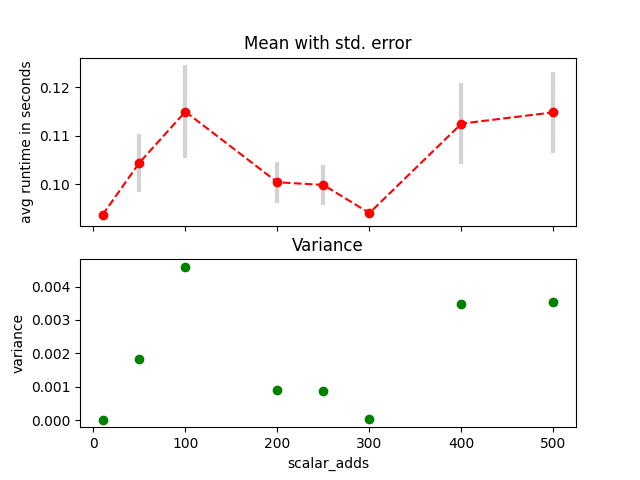
\includegraphics[width=0.49\linewidth]{../performance_analysis/runtime_scalar_additions.png}
    \caption{Avg Runtime and Dataflow change based on the number of Scalar Addtions}
    \label{fig:scalar_add}
\end{figure}


\begin{figure}[h!]
    \centering
    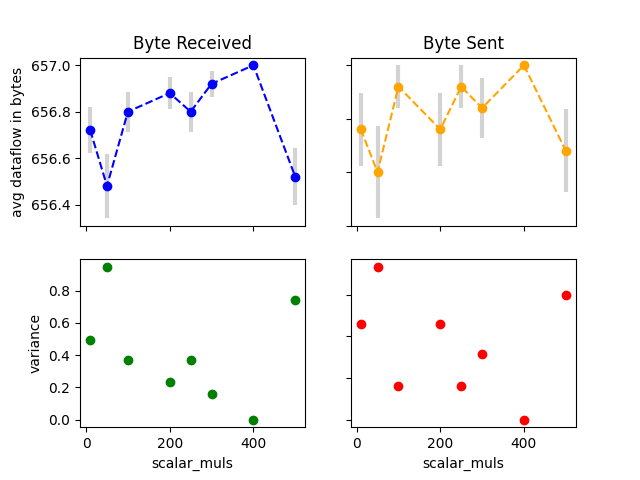
\includegraphics[width=0.49\linewidth]{../performance_analysis/dataflow_scalar_multiplications.png}
    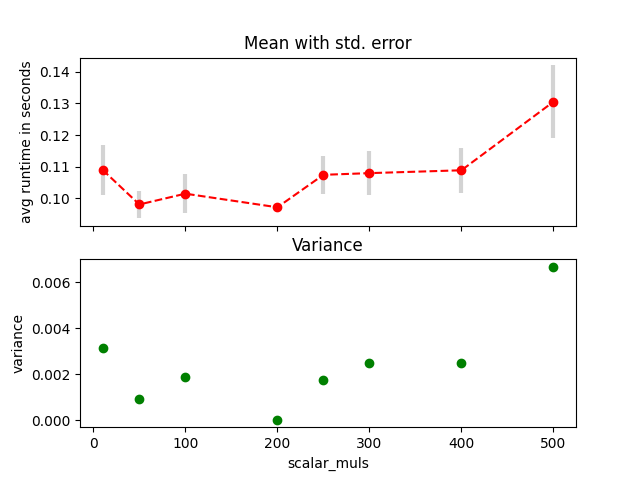
\includegraphics[width=0.49\linewidth]{../performance_analysis/runtime_scalar_multiplications.png}
    \caption{Avg Runtime and Dataflow change based on the number of Scalar Multiplications}
    \label{fig:scalar_mult}
\end{figure}


\subsection{Effect on of the number of parties \ref{fig:num_parties}}
This specific test was run on an expression containing 60 secrets in the form: $s_1 + s_2 + s+_3 \dots s_{30} * s_{31} *
s_{32} * \dots*  s_{60}$

For, the data-flow we can see a linear increase for the number of bytes received, and a logarithmic-like increase for the
number of bytes sent.
The linear increase in bytes received is expected as the number of inputs (for one party) to the Beaver Protocol required to perform the secret to secret multiplication is linear in the number of parties.
As far as the bytes sent are concerned, the dominant part of the protocol is represented by the \texttt{init\_secret\_sharing} function where shares are sent to other parties.
The logarithmic-like increase in bytes sent can be explained by the ratio between the number of shares to send vs the
number of parties to send these shares to.
More specifically, the number of shares sent is: $\frac{60*(n-1)}{n}$.
The computational time increases exponentially as O($n^2$), reflecting the complexity in terms of shares to be fetched during the Beaver Protocol ($n$ parties fetching $2*(n-1)$ messages).


\subsection{Effect of number of Secret Additions \ref{fig:num_additions}}

For the dataflow we can see a linear increase in bytes sent and received.
The runtime increases linearly as well.

\subsection{Effect of Number of Secret Multiplication \ref{fig:num_multiplications}}
Both dataflow and computation time show a linear increase.

\subsection{Effect of Number of scalars \ref{fig:scalar_add},\ref{fig:scalar_mult}}
For these we see no significant difference in the number of bytes sent and received.
this behaviour is explained by the fact that scalars are constants and shared across all parties, meaning that no network
I/O is required to perform the computation.
The only slight differences shown by the variance and error bars are caused by the serialization of the data.
When it comes to the runtime we can see a slight inconsistent increase.
This is probably due to the fact that since these operations do not require any Network I/O, they are more
prone to the CPU computational noise.

\section{Application}
A realistic use case for the framework is computing the average GPA of the semester among $n$ students. The circuit would be the following:
\[f = \frac{\sum_{i=1}^{n_{parties}}(\sum_{j=1}^{n_{grades}}grade_{ij}*ects_{ij})}{\sum_{i,j}ects_{ij}}\]
In the implementation, students who do not want to reveal their grades and credits will exploit the \texttt{Secret()} class, otherwise they will make use of \texttt{Scalar()}.
In order to avoid defining the division modulo $q$, the numerator and denominator of the fraction will be evaluated as two separate expressions, and then the division will be locally computed by each party.
As far as privacy flaws are concerned, there is again the problem of a passive adversary being capable of inferring a target party's secret (in particular the most sensitive information, the grade) if she manages to compromise all but one secrets.
Also, taking into account adversary's background knowledge (such as a student having access to the list of other students enrolled in her same course), a mitigation to this problem could be to add noise to the output so to achieve $\epsilon$ \textit{differential-privacy}. Nevertheless, taking into account the narrow range of values the mean can assume, $[0,6]$, this solution will probably compromise the utility of the computation.  
\bibliographystyle{IEEEtran}
\bibliography{bib}
\end{document}
